\documentclass{article}

\usepackage[final]{corl_2026}
\usepackage{booktabs}
\usepackage{graphicx}
\usepackage{amsmath}
\usepackage{amssymb}
\usepackage{xcolor}
\usepackage{url}

\title{Reward Shaping and Opponent Curricula for Sparse-Reward Multi-Agent Play in SoccerTwos}

\author{
  Chuye Zhang \\
  Georgia Institute of Technology \\
  \texttt{czhang883@gatech.edu} \\
  \And
  Jianuo Qiu \\
  Georgia Institute of Technology \\
  \texttt{jqiu317@gatech.edu} \\
}

\begin{document}
\maketitle

\begin{abstract}
We apply delta-based reward shaping and a four-stage opponent curriculum to PPO in the SoccerTwos environment. Reward shaping alone bootstraps learning within $0.25$M steps and reaches $8/10$ wins versus the CEIA baseline; our submitted agent LUCKETS\_AGENT adds a redesigned four-stage curriculum (trained over a stitched $35.8$M-step three-segment chain) and beats the shaping-only variant $7/10$ in head-to-head play. Pure PPO self-play without shaping scores \emph{zero} goals in $10$ matches, confirming that the reward signal---not the self-play structure---is the primary bottleneck. We also report a first-attempt curriculum that failed to advance past Stage~$0$ due to an opponent-policy mapping bug, which directly motivated the redesign.
\end{abstract}

\begin{center}
\textbf{Code:} \url{https://github.com/ZhangChuye/soccer-twos-starter-18}\\
\textbf{Submitted agent} (single agent, covers all rubric criteria):
\texttt{LUCKETS\_AGENT} \;---\; Policy performance, Reward modification, Curriculum learning.
\end{center}

\keywords{Multi-agent RL, reward shaping, curriculum learning, PPO, SoccerTwos}

%===============================================================================
\section{Overview}

Raw PPO on SoccerTwos faces two obstacles: (i) goals are rare, so the sparse $\pm 1$ reward gives almost no gradient signal in early training; and (ii) a self-play opponent that is always ``yourself'' produces a non-stationary target that offers little stable learning signal once both sides converge on a trivial strategy.
We address (i) with small delta-based dense reward terms that fire on every step without changing the optimal policy, and (ii) with a four-stage opponent curriculum that starts against a random opponent and gradually escalates to the CEIA baseline and then self-play~\citep{Bengio2009Curriculum}.
We run three configurations---reward shaping only, pure sparse self-play, and the combined agent---to isolate each contribution.

%===============================================================================
\section{Method}
\label{sec:method}

\textbf{Algorithm and library.}
All runs use Ray RLlib~\citep{Liang2018RLlib} with the PPO trainer~\citep{Schulman2017PPO} (Ray 1.4.0, PyTorch, two-layer MLP $[256,256]$, ReLU). Hyperparameters: Appendix~\ref{sec:hp}.

\textbf{Reward modification.}
The default environment returns $\pm 1$ only at goals plus a small per-step penalty. We wrap it with \texttt{RewardShaperWrapper} (\texttt{utils.py}) which adds two dense terms each step:
\begin{equation}
r^{\text{prox}}_t(i) = \alpha_{\text{prox}}\bigl(d_{t-1}(i)-d_t(i)\bigr), \qquad
r^{\text{prog}}_t(i) = \alpha_{\text{prog}}\bigl(x^{\text{ball}}_t - x^{\text{ball}}_{t-1}\bigr)\,\mathrm{sign}(\mathrm{team}(i))
\label{eq:shaping}
\end{equation}
where $d_t(i)=\lVert p^{\text{player}}_t(i)-p^{\text{ball}}_t\rVert_2$ and $x^{\text{ball}}$ is the ball's forward coordinate; $\alpha_{\text{prox}}{=}0.02$, $\alpha_{\text{prog}}{=}0.05$.
Both terms are \emph{deltas}: agents are rewarded only for \emph{approaching} the ball and \emph{moving} it toward the opponent goal, not for already being close---so the shaping is nearly potential-based~\citep{Ng1999RewardShaping}, preserving the optimal policy.
\textit{Motivation:} the sparse goal reward fires on $<\!1\%$ of steps, so PPO's gradient is dominated by advantage variance; per-step deltas bootstrap the agent past the ``nothing happens'' phase efficiently.

\textbf{Opponent curriculum (LUCKETS\_AGENT).}
A \texttt{CurriculumCallback} remaps orange-team policies in four stages: \emph{(0)~Random:} both $\to$ \texttt{opp\_rand}; \emph{(1)~Hybrid:} agent~2 $\to$ \texttt{opp\_base} (CEIA), agent~3 $\to$ \texttt{opp\_rand}; \emph{(2)~Baseline:} both $\to$ \texttt{opp\_base}; \emph{(3)~Self-play:} both $\to$ \texttt{opp\_self} (frozen learner snapshot).
Promotion requires win rate $\ge 0.80$ for $3$ consecutive iterations.
The current stage is persisted to \texttt{.curriculum\_stage} and read by every Ray worker on each rollout.
\textit{Motivation:} a policy trained only against a random opponent has a narrow occupancy distribution; directly switching to the CEIA baseline collapses training. The ramp keeps the learning problem just difficult enough to make progress at each stage.

%===============================================================================
\section{Experimental Results}
\label{sec:result}

\textbf{Exploration path} (Fig.~\ref{fig:training}).
\emph{Phase~1 (Agent~2):} sparse PPO self-play (\texttt{67194}, $2.4$M steps) scored zero goals.
\emph{Phase~2 (Agent~1):} adding shaping vs.\ a frozen random opponent (\texttt{a6c6d}, $10$M steps) crossed $0.9$ win rate at $0.25$M and reached $8/10$ vs.\ CEIA.
\emph{Phase~3:} a first-attempt curriculum with a single shared \texttt{opponent} policy (\texttt{7b8e4}, $15$M steps) hit $0.99$ win rate but stayed at Stage~$0$ throughout---our promotion gate fired but the single-policy design could not be remapped at runtime in RLlib's worker config.
\emph{Phase~4 (LUCKETS\_AGENT):} we redesigned the curriculum with three separate opponent policies (\texttt{opp\_rand}, \texttt{opp\_base}, \texttt{opp\_self}) selected by \texttt{policy\_mapping\_fn} from a stage file persisted across Ray workers, and trained three resumed segments: Stage~$0\!\to\!1$ ($0\!-\!15$M, \texttt{c33b8}), Stage~$1\!\to\!2$ ($15\!-\!20.8$M, \texttt{6eb9a}), Stage~$2\!\to\!3$ ($20.8\!-\!35.8$M, \texttt{02fdb}). \texttt{checkpoint-600} of \texttt{02fdb} ships as LUCKETS\_AGENT.

\begin{figure}[t]
\centering
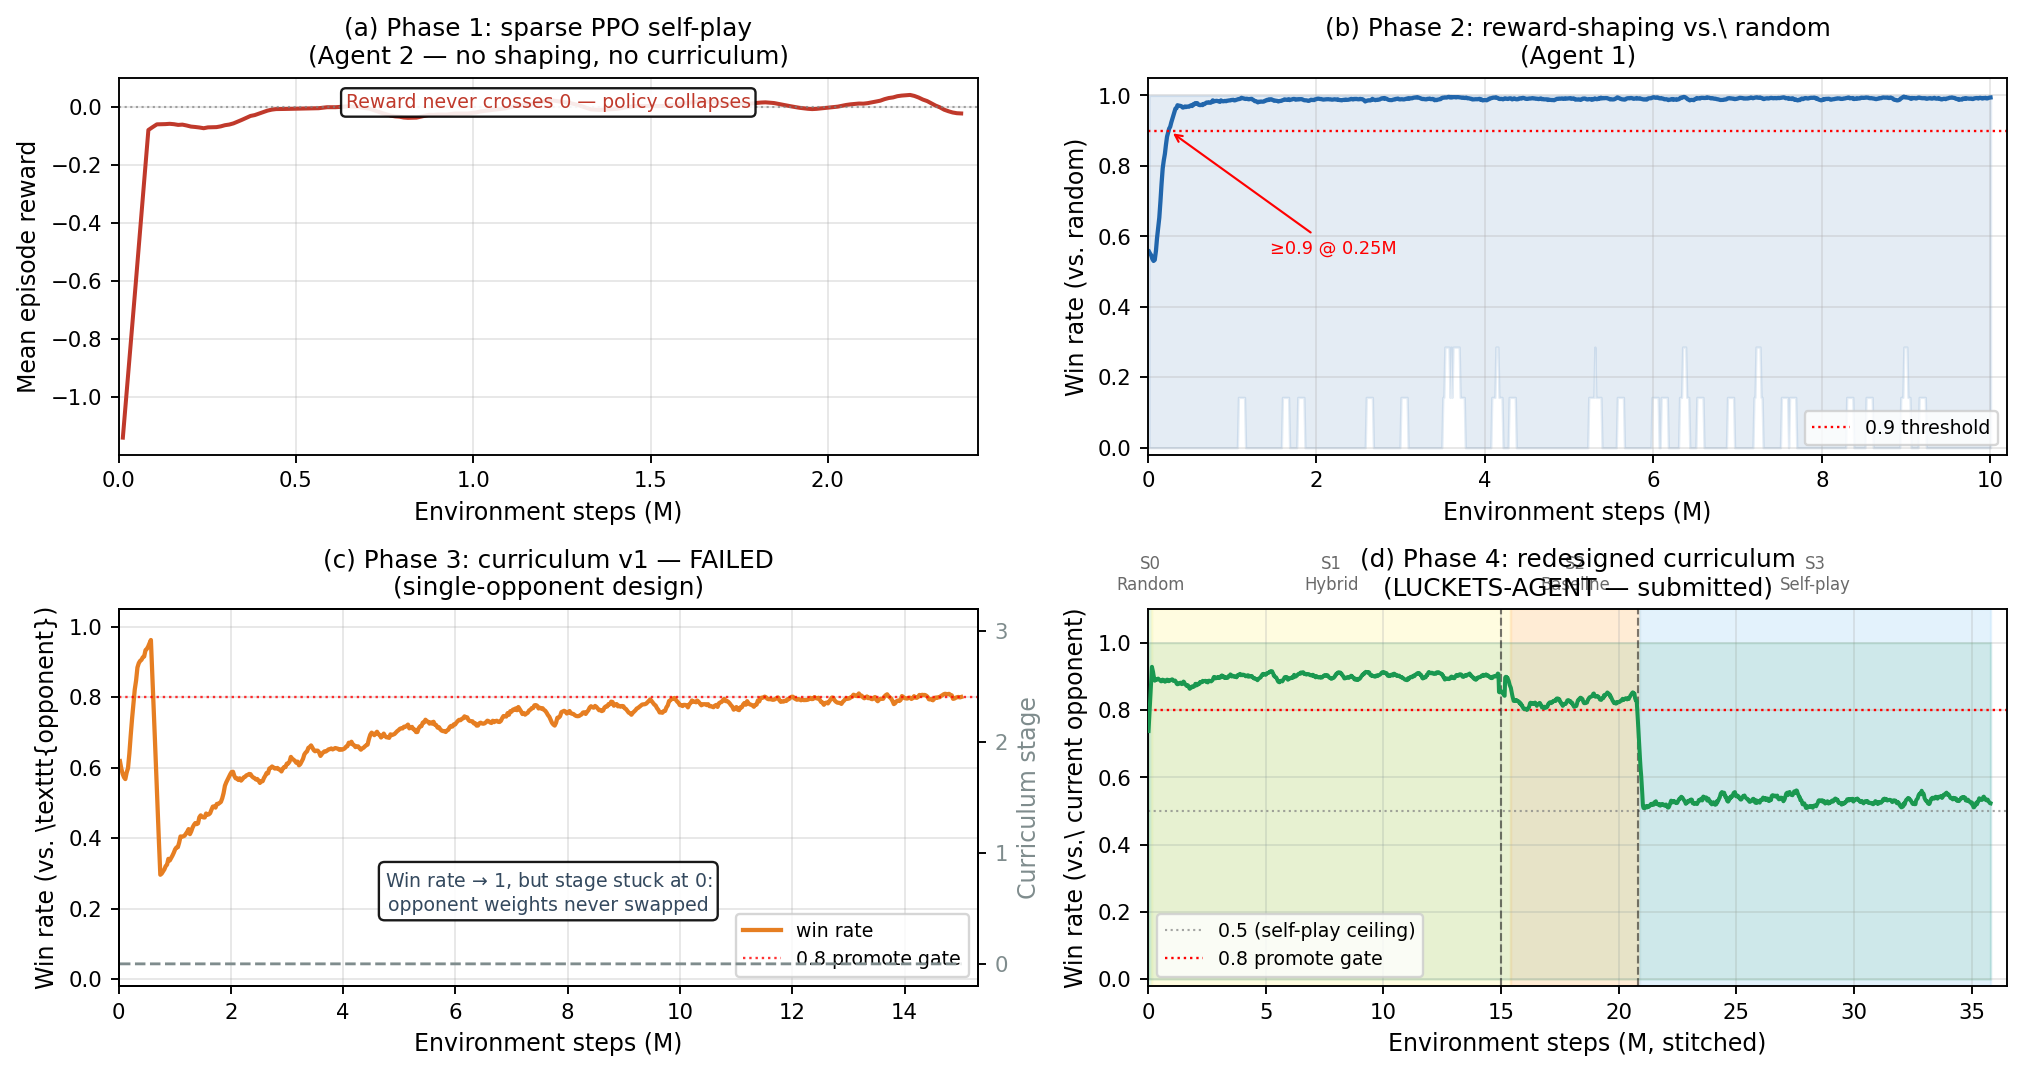
\includegraphics[width=\textwidth]{fig_training_all.png}
\caption{\textbf{Training curves for all four experiments.}
(a)~\emph{Phase~1, sparse self-play} (\texttt{67194}, $2.4$M steps): episode reward never crosses $0$.
(b)~\emph{Phase~2, reward shaping vs.\ random} (\texttt{a6c6d}, $10$M steps): win rate $\ge\!0.9$ within $0.25$M steps, saturating near $1.0$.
(c)~\emph{Phase~3, curriculum~v1 — failed} (\texttt{7b8e4}, $15$M steps): win rate climbs but \emph{curriculum stage remains 0 throughout} (right axis) because the single-opponent design cannot swap weights at runtime.
(d)~\emph{Phase~4, redesigned curriculum} (\texttt{c33b8 + 6eb9a + 02fdb}, $35.8$M steps stitched): colored backgrounds mark the four curriculum stages; black dashed verticals are the two segment resumes; red dotted is the $0.8$ promotion gate; grey dotted is the $0.5$ self-play symmetric ceiling.}
\label{fig:training}
\end{figure}

\textbf{Head-to-head evaluation.}
We ran $10$ headless matches per pairing ($1{,}000$ step timeout, \texttt{explore=False}).
Table~\ref{tab:eval} reports win/loss/draw from team~0's perspective.
Agent~3 (LUCKETS) wins $8/10$ versus CEIA ($2$ losses, $0$ draws) and beats Agent~1 $7\text{-}1\text{-}2$.
Agent~1 also wins $8/10$ versus CEIA but with $2$ draws instead of losses, indicating Agent~3 is more aggressive but occasionally over-commits.
Agent~2 draws all $10$ matches against the example player and loses all $10$ to CEIA.

\begin{table}[t]
\centering
\small
\begin{tabular}{lcccc}
\toprule
 & Ex.\ player & CEIA & Ag.~1 (rew.\ shaped) & Ag.~2 (self-play) \\
\midrule
\textbf{Agent~1}: reward-shaped  & $10/0/0$ & $8/0/2$ & ---     & $10/0/0$ \\
\textbf{Agent~2}: self-play      & $0/0/10$ & $0/10/0$ & ---    & ---      \\
\textbf{Agent~3}: LUCKETS (ours) & $10/0/0$ & $8/2/0$ & $7/1/2$ & $10/0/0$ \\
\bottomrule
\end{tabular}
\caption{\textbf{Head-to-head record} (wins / losses / draws), $10$ matches per pairing.
Each row is the blue team; column is the orange opponent.
``---'' = symmetric duplicate not run.}
\label{tab:eval}
\end{table}

\begin{figure}[t]
\centering
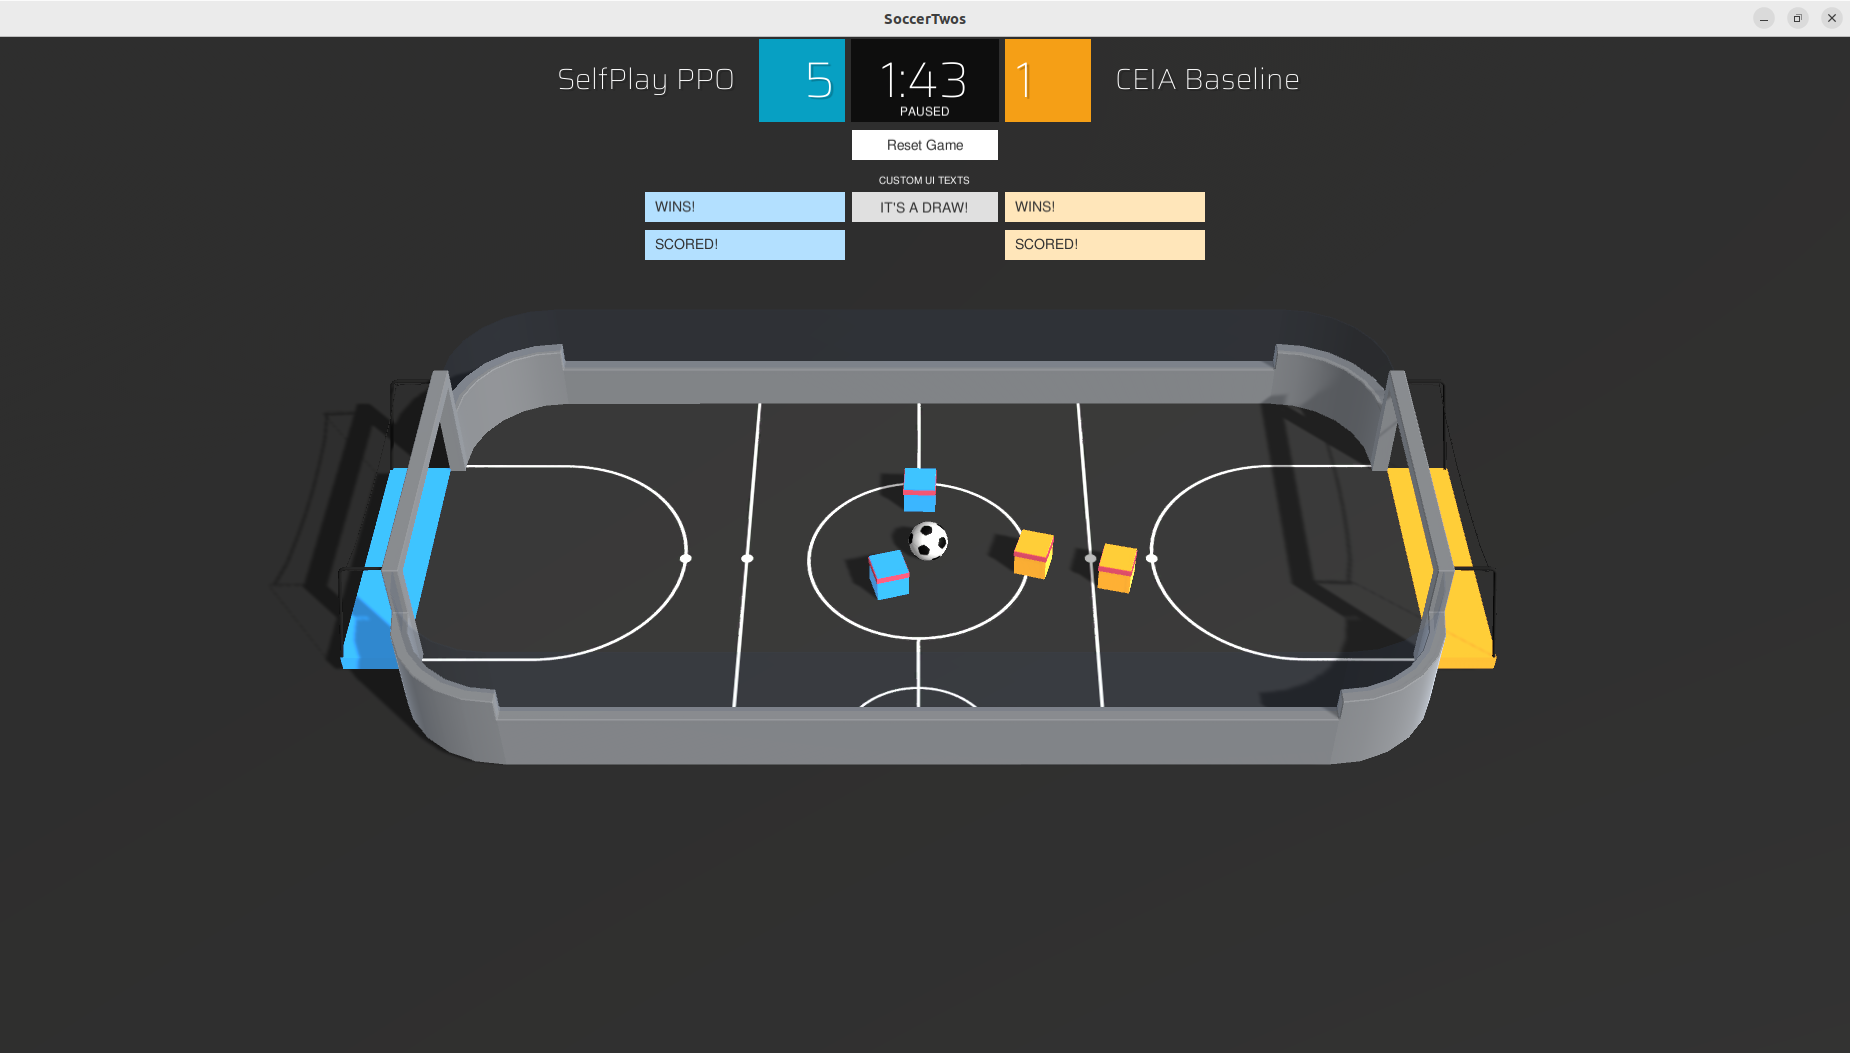
\includegraphics[width=0.40\textwidth]{overall_figure.png}
\caption{\small LUCKETS\_AGENT (blue) vs.\ CEIA baseline (orange) during evaluation; score 5--1 mid-game.}
\label{fig:game}
\end{figure}

%===============================================================================
\section{Analysis and Discussion}
\label{sec:analysis}

\textbf{Reward shaping.} \emph{Result: higher reward and faster convergence.}
With sparse reward, the policy gradient is dominated by variance because goal events fire on $<\!1\%$ of steps. The delta form of Eq.~\ref{eq:shaping} converts every step into a small informative signal without changing the optimal policy, and using \emph{deltas} (not absolute values) avoids the ball-chasing attractor an absolute-distance reward would create. This is why Agent~1 reaches $0.9$ win rate within $0.25$M steps while Agent~2 (sparse) never scores.

\textbf{Curriculum.} \emph{Result: higher peak performance.}
Agent~3 beats Agent~1 $7\text{-}1\text{-}2$ despite using identical shaping, because a policy trained only against random opponents has a narrow occupancy distribution that is partly off-support against CEIA defense. Stages~1--2 shift training toward that distribution, Stage~3 keeps it expanding. Fig.~\ref{fig:training}d shows the expected staircase: win rate drops at each stage advance and recovers. Curriculum~v1 failed for an architectural reason: with a single shared \texttt{opponent} policy, weight swaps mid-run require copying tensors through every Ray worker, but our naive callback only updated the driver's copy. The fix is to declare all three opponent policies up front and route each agent ID through \texttt{policy\_mapping\_fn} from a worker-shared stage file.

\textbf{Pure self-play failure.}
Without shaping, no player generates a scoring trajectory early enough to provide a gradient; both sides converge on a trivial idle strategy with zero goals, entropy collapses, and rotating snapshots cannot perturb the fixed point because the reward signal for escaping it is identically zero.

\textbf{Limitations.} Both agents stop at $8/10$ vs.\ CEIA, not a decisive $9/10$; the two Agent~3 losses suggest over-committing on offense. Shaping ignores teammate position, so no passing incentive is learned. A symmetric demotion rule (promote at $\ge 0.8$, demote at $\le 0.4$) is the most likely next improvement.

%===============================================================================
\acknowledgments{We thank the course staff for the SoccerTwos starter kit~\citep{Oliveira2021SoccerTwos} and the CEIA baseline, and the Georgia Tech PACE team for cluster access.}

\bibliography{references}

%===============================================================================
\appendix
\section{Hyperparameters}
\label{sec:hp}

\begin{table}[h]
\centering
\small
\begin{tabular}{ll}
\toprule
Hyperparameter & Value \\
\midrule
Algorithm                  & PPO (Ray RLlib 1.4.0, PyTorch) \\
Policy/value network       & MLP $[256,256]$, ReLU, shared trunk + value head \\
Learning rate              & $3\times 10^{-4}$ \\
Discount $\gamma$          & $0.995$ \\
GAE $\lambda$              & $0.95$ \\
PPO clip $\epsilon$        & $0.2$ \\
Entropy coefficient        & $0.01$ \\
Value-loss coefficient     & $0.5$ \\
SGD minibatch / epochs     & $512$ / $10$ \\
Train batch size           & $12{,}000$ \\
Rollout fragment           & $1{,}000$ \\
Workers $\times$ envs/wkr  & $12\times3=36$ \\
Total env steps            & $\sim$$10$M (Agent~1); $\sim$$2.4$M (Agent~2); $\sim$$35.8$M (Agent~3) \\
\midrule
Shaping $\alpha_{\text{prox}}$ (Agents 1, 3) & $0.02$ \\
Shaping $\alpha_{\text{prog}}$ (Agents 1, 3) & $0.05$ \\
Promotion gate (Agent 3)   & win rate $\ge 0.80$ for $3$ consecutive iters \\
\bottomrule
\end{tabular}
\caption{Final-run hyperparameters. Shaping coefficients are zero for Agent~2.}
\label{tab:hp}
\end{table}

\end{document}
